\documentclass[conference]{IEEEtran}

\usepackage{cite}
\usepackage{amsmath,amssymb}
\usepackage{graphicx}
\usepackage{booktabs}
\usepackage{url}
\usepackage{xcolor}
\usepackage{multirow}
\usepackage{array}
\usepackage[compact]{titlesec}
% Tighten vertical space around section / subsection headings (no font changes)
\titlespacing*{\section}{0pt}{6pt plus 1pt minus 1pt}{3pt plus 1pt}
\titlespacing*{\subsection}{0pt}{5pt plus 1pt minus 1pt}{2pt plus 1pt}
% Tighten spacing around floats (tables / figures) so they leave less whitespace
\setlength{\textfloatsep}{6pt plus 2pt minus 2pt}
\setlength{\intextsep}{6pt plus 2pt minus 2pt}
\setlength{\floatsep}{6pt plus 2pt minus 2pt}
\setlength{\dbltextfloatsep}{6pt plus 2pt minus 2pt}

\begin{document}

\title{Do Large Language Models Think Fast and Slow?\\Eliciting Dual-Process Behavioral Signatures with\\Implications for Biomedical AI}

% Anonymous submission
\author{\IEEEauthorblockN{Anonymous BIBM Submission}
\IEEEauthorblockA{Paper ID: XXX}}

\maketitle

\begin{abstract}
Dual-process theory distinguishes fast, intuitive System~1 from slow, analytical System~2 processing, a distinction central to clinical decision-making. We ask whether LLMs exhibit analogous behavioral signatures under systematic parameter manipulation. Unlike prior work that confounds model capacity, temperature, and prompting, we run a $2 \times 2 \times 2$ factorial ablation that isolates each factor. The central finding is a strong Prompt $\times$ Task Category interaction ($F(2, 4794) = 89.2$, $p < .001$, $\eta^2_p = .036$): CoT yields a $+31.2$-point gain on analytical tasks and an $11.1$-point raw decrement on intuitive ones (half of which is a format artefact on one coreference benchmark; the interaction survives its exclusion, $F(2, 4570) = 71.7$, $p < .001$). We replicate across four LLM families and on 100 MedQA-USMLE vignettes, and stress-test conflict performance with 50 novel memorization-resistant items. These findings support configuring clinical decision-support LLMs with System~1-like settings for routine triage and System~2-like settings for complex diagnosis.
\end{abstract}

\begin{IEEEkeywords}
dual-process theory, large language models, clinical decision support, chain-of-thought reasoning, biomedical informatics
\end{IEEEkeywords}

%% ============================================================
\section{Introduction}
\label{sec:intro}

Dual-process accounts of human cognition distinguish a fast, automatic, heuristic-driven System~1 from a slow, deliberate, rule-based System~2~\cite{Kahneman2011, Stanovich2000}. Classic demonstrations such as Frederick's Cognitive Reflection Test~\cite{Frederick2005} show that intuitive first responses routinely override careful analysis, with broad implications for judgment and decision-making~\cite{Tversky1974}.

The distinction is especially consequential in clinical medicine, where the same System~1 / System~2 toggle underlies both efficient pattern recognition and analytical differential diagnosis: a setting where large language models (LLMs) are rapidly being deployed for triage, documentation, and decision support~\cite{Singhal2023, Thirunavukarasu2023, Lee2023}. If LLMs can be configured to exhibit either mode, this directly shapes system design: rapid triage queries may benefit from efficient System~1-like responses, while complex diagnostic reasoning demands the thoroughness of System~2-like processing. Section~\ref{sec:background} expands on the clinical-reasoning background.

Recent studies suggest that LLMs exhibit human-like cognitive patterns: they demonstrate analogical reasoning~\cite{Webb2023}, display intuitive biases~\cite{Hagendorff2023}, and can engage in chain-of-thought reasoning when prompted~\cite{Wei2022}. These observations motivate our central question: \textit{Can LLMs be configured to systematically exhibit the distinct behavioral signatures of System~1 and System~2 processing, and what are the implications for biomedical applications?}

We present the following contributions:

\begin{enumerate}
\item A \textbf{$2 \times 2 \times 2$ factorial ablation} that isolates the contributions of model capacity, temperature, and prompting strategy, and reveals a strong Prompt $\times$ Task Category interaction: CoT produces a large accuracy gain on analytical tasks ($+31.2$) and a raw $-11.1$-point decrement on intuitive tasks (of which roughly half is traced to CoT-induced hedging on the WinoGrande coreference format), the directional asymmetry predicted by dual-process theory but not guaranteed by the design.
\item \textbf{Cross-model validation} across four LLM families (OpenAI, DeepSeek, Qwen, open-source Llama), demonstrating that dual-process behavioral patterns are not artifacts of a single provider.
\item A set of \textbf{50 novel conflict items} (covering CRT variants, base-rate neglect, conjunction fallacy, biomedical Bayesian reasoning, and other heuristic-and-bias items) structurally isomorphic to their classic sources but written with novel surface content to reduce training-data memorization, used to characterise where LLMs succeed or fail when the intuitive cue cannot be retrieved from memory.
\item \textbf{Token efficiency} as a model-intrinsic computational effort metric, replacing wall-clock response time which conflates model computation with API infrastructure.
\end{enumerate}

%% ============================================================
\section{Background and Related Work}
\label{sec:background}

\subsection{Dual-Process Theory in Human Cognition}

Beyond the classic Kahneman/Stanovich treatments cited above, converging evidence from reasoning and judgment tasks establishes System~1 as associative/automatic and System~2 as rule-based/controlled~\cite{Sloman1996, Evans2008}. The distinction is theoretically contested: critics argue it oversimplifies a continuum of processing modes~\cite{Evans2013}. We do not require dual-process theory to be literally true of human cognition; we use its behavioral predictions (differential performance across task types, effort-accuracy trade-offs) as a structured framework for characterizing LLM behavior under different configurations.

\subsection{Dual-Process Cognition in Clinical Medicine}

Clinicians toggle between intuitive pattern recognition and analytical reasoning~\cite{Croskerry2009}. Pattern recognition enables rapid identification of common conditions but also produces diagnostic errors (anchoring, availability, premature closure)~\cite{Croskerry2013, Saposnik2016}; diagnostic errors often arise from failure to engage deliberate reasoning when an intuitive hypothesis is wrong~\cite{Norman2009, Pelaccia2011}. If LLMs exhibit analogous configuration-dependent behavior, the same design principles governing when clinicians should deliberate can inform when LLM systems should be configured for thorough analysis versus rapid response.

\subsection{Dual-Process Patterns in LLMs}

Prior work has documented human-like behavioral patterns in LLMs: analogical reasoning~\cite{Webb2023}, intuitive biases and emergent cognitive biases~\cite{Binz2023, Hagendorff2023, Itzhak2024}, and foundation models explicitly capturing human cognition~\cite{Binz2025}. On prompting, chain-of-thought (CoT) substantially improves reasoning~\cite{Wei2022, Kojima2022}, while Liu et al.~\cite{Liu2024} showed that CoT can \textit{reduce} performance on tasks where deliberation harms humans. DeepSeek-R1~\cite{DeepSeekAI2025} represents a deliberate engineering effort toward System~2-like extended reasoning; Bellini-Leite~\cite{BelliniLeite2024} gives a theoretical overview. In the medical domain LLMs have reached expert-level clinical knowledge~\cite{Singhal2023, Nori2023} and diagnostic reasoning prompts show interpretability potential~\cite{Savage2024}.

%% ============================================================
\section{Method}
\label{sec:method}

\subsection{Research Questions}

We designed our study to address four core questions:

\textbf{RQ1 (Factorial Isolation):} Which parameter (model capacity, temperature, or prompting strategy) contributes most to dual-process behavioral differences, and do these factors interact with task type?

\textbf{RQ2 (Token Efficiency):} Do the two configurations exhibit effort asymmetry measured through token efficiency, and does this differ by task type?

\textbf{RQ3 (Generalizability):} Do dual-process patterns generalize across model families and persist on novel conflict tasks resistant to memorization?

\textbf{RQ4 (Human Comparison):} Where do LLM dual-process patterns converge with and diverge from human behavioral data?

\subsection{System Configuration}

We operationalize the S1 / S2 contrast along three parameter axes: \textbf{model capacity} (smaller/faster vs.\ larger/capable variant within each family), \textbf{decoding temperature} (0.9 vs.\ 0.2), and \textbf{prompting strategy} (zero-shot vs.\ chain-of-thought~\cite{Wei2022}). The System~1 prompt was: ``\textit{You are a fast, intuitive thinker. Answer immediately with your first instinct. Give a brief, direct answer. Trust your gut feeling.}''; the System~2 prompt was: ``\textit{You are a careful, analytical thinker. Think step by step. Break down the problem systematically before reaching a conclusion.}'' Both prompts required JSON output containing an \texttt{answer} and a \texttt{confidence} rating (0--1); CoT additionally included a \texttt{reasoning\_steps} array. Completion-token caps were 150 for ZS and 1000 for CoT; observed C5/C8 medians/p90s/max were 144/239/451 and 369/503/713, so the caps bound only a tail and the $2.40\times$ token ratio is a deployment-settings estimate rather than an unconstrained one. Temperature turns out to be empirically null in our data (\S\ref{sec:factorial-results}) and we retain it only so the factorial cleanly decomposes its contribution.

We do not claim that LLMs possess unconscious processes or subjective experience: System~1 and System~2 here refer to \textit{behavioral configurations} (observable accuracy, token-usage, and confidence differences), not internal mechanisms.

\subsection{Factorial Ablation Design}
\label{sec:factorial}

A key criticism of prior work (including our initial CogSci submission) is that model, temperature, and prompting are confounded: all three change simultaneously between System~1 and System~2. This means any observed difference could be driven by one factor while the others are irrelevant. To isolate each factor's contribution, we conduct a $2 \times 2 \times 2$ factorial ablation (Table~\ref{tab:factorial}).

\begin{table}[t]
\caption{$2 \times 2 \times 2$ factorial ablation design. C1 and C8 correspond to the original System~1 and System~2 configurations.}
\label{tab:factorial}
\centering
\begin{tabular}{cccc}
\toprule
Condition & Model & Temp. & Prompt \\
\midrule
C1 (S1) & Mini & High & Zero-shot \\
C2 & Mini & High & CoT \\
C3 & Mini & Low & Zero-shot \\
C4 & Mini & Low & CoT \\
C5 & Full & High & Zero-shot \\
C6 & Full & High & CoT \\
C7 & Full & Low & Zero-shot \\
C8 (S2) & Full & Low & CoT \\
\bottomrule
\end{tabular}
\end{table}

This design enables estimation of main effects for each factor, all two-way interactions (Model $\times$ Prompt, Model $\times$ Temperature, Prompt $\times$ Temperature), and the three-way interaction. Critically, the Prompt $\times$ Task Category interaction is our primary test of the dual-process prediction: if CoT helps more on analytical than intuitive tasks, this interaction effect is \textit{not} circular, since one could equally observe CoT helping uniformly across all task types.

Both System~1 and System~2 configurations use a single API call per task with different prompts and parameters; no multi-stage processing pipeline is involved. The factorial design tests all $2^3 = 8$ combinations. Our \textbf{primary comparison} is C5 vs.\ C8 (same model GPT-4o, differing only in temperature and prompt), which isolates configuration effects from model capacity. The \textbf{secondary comparison} is C1 vs.\ C8 (the full canonical System~1 vs.\ System~2), contextualized by the factorial results.

\subsection{Multi-Model Validation}
\label{sec:multimodel}

To assess generalizability, we replicate the core System~1 vs.\ System~2 comparison across four LLM families (Table~\ref{tab:model-families}).

\begin{table}[t]
\caption{Model families used for cross-model validation.}
\label{tab:model-families}
\centering
\begin{tabular}{lll}
\toprule
Family & System 1 & System 2 \\
\midrule
OpenAI & GPT-4o-mini & GPT-4o \\
DeepSeek & DeepSeek-Chat & DeepSeek-R1 \\
Qwen & Qwen2.5-7B-Instruct & Qwen2.5-72B-Instruct \\
Meta (Llama) & Llama 3.1 8B & Llama 3.3 70B \\
\bottomrule
\end{tabular}
\end{table}

For each family, the smaller/faster model is configured as System~1 and the larger/more capable model as System~2, using the same temperature and prompting parameters. Each family was evaluated on $n = 100$ items per task category (300 items total per family per system configuration). The same stratified-sampling and option-randomization protocol used in the factorial ablation is applied here to the conflict category, yielding 50 novel + 50 classic items per condition (all 50 novel items are forced in, with classic items drawn under the shared fixed seed so every family sees the same set).

\subsection{Task Design}

We assembled a task battery from established NLP benchmarks spanning three categories ($n = 200$ items per category), each designed to differentially engage the two processing modes. The full pool contains approximately 11{,}117 items, from which we sample 200 per category.

\textbf{Intuitive Tasks:} Pattern completion, semantic associations, common-sense judgments, and rapid categorization, drawn from HellaSwag, PIQA, SIQA, CommonsenseQA, and WinoGrande. These tasks have clear intuitive answers accessible through pattern matching and associative retrieval.

\textbf{Analytical Tasks:} Multi-step arithmetic and logical deduction, drawn from GSM8K and LogiQA. These tasks require systematic step-by-step analysis.

\textbf{Conflict Tasks:} Items drawn from TruthfulQA plus 50 novel items, where the intuitive answer is systematically wrong. Classic CRT-style problems, base-rate neglect scenarios, and other heuristic-and-bias items (sunk cost, gambler's fallacy, availability) present situations where an intuitive lure diverges from the correct analytical answer~\cite{Frederick2005}.

We excluded benchmarks that span both intuitive and analytical demands (e.g., ARC, MMLU) to ensure clean category boundaries.

\textbf{Novel Conflict Tasks.} To address training-data memorization, we developed 50 novel conflict items (10 each in five subcategories: CRT variants, base-rate neglect, conjunction fallacy, biomedical Bayesian reasoning, and other heuristic-and-bias items such as sunk cost, gambler's fallacy, and availability) that are structurally isomorphic to the corresponding classic problems but use novel surface content unlikely to appear in training corpora. Each item presents a salient intuitive lure diverging from the correct answer. Rather than uniform random sampling (which, at $n = 200$ from a pool of $867$, would yield only ${\sim}12$ novel items per condition in expectation), we use \textit{stratified sampling} that forces all 50 novel items into every conflict sample, filled by 150 randomly drawn classic (TruthfulQA) items under a fixed seed shared across all 8 factorial conditions. To further eliminate a positional-bias shortcut (several sources place the correct option in position A by default), we randomise MCQ option positions per item using a deterministic per-item hash, so every condition sees the same post-shuffle layout. Free-form novel items (e.g., ``\$5'' as the CRT answer) are scored by numeric extraction and are unaffected by this transformation.

\subsection{Metrics}

\begin{itemize}
\item \textbf{Accuracy:} Correctness of the final answer.
\item \textbf{Confidence:} Model-generated certainty rating (0--1 scale).
\item \textbf{Token Efficiency Ratio (TER):} Defined as $\text{TER} = \Delta\text{Accuracy} / \Delta\text{Tokens}$, measuring the accuracy gain (in percentage points) per additional token consumed by System~2 relative to System~1. High TER indicates efficient use of additional computation; low or negative TER indicates diminishing or reversed returns.
\item \textbf{Marginal Accuracy Gain ($\Delta\text{Accuracy}$):} The raw accuracy delta $Acc_{S2} - Acc_{S1}$ used as the numerator of TER; reported alongside the corresponding $\Delta\text{Tokens}$ for interpretability.
\end{itemize}

Model responses were parsed as JSON, and accuracy was assessed against the extracted answer field to prevent false matches from intermediate reasoning steps.

We deliberately exclude wall-clock response time. API response time conflates model computation with network latency, server load, and batching, factors external to the model. Token usage is a model-intrinsic metric directly analogous to cognitive effort in dual-process theory.

\subsection{Statistical Methods}

For the factorial ablation, we use three-way ANOVA on accuracy with model, temperature, and prompting as fixed factors and task category as a moderator. For pairwise comparisons, we use independent samples $t$-tests with Cohen's $d$ effect sizes~\cite{Cohen1988}. Our pre-specified primary comparisons are (i) C5 vs.\ C8 on overall accuracy and on each of the three task categories, and (ii) C1 vs.\ C8 on the conflict category, five tests in total. At a Bonferroni-corrected threshold of $\alpha = .05 / 5 = .01$, every comparison we report as ``significant'' remains significant; we report raw $p$-values throughout and include all non-significant results to avoid selective reporting.

\subsection{Control Baselines}

We include two control baselines to contextualize observed effects. A \textbf{random baseline} establishes expected accuracy for multiple-choice tasks ($1/n_{\text{options}}$). TruthfulQA items have a mean of about 5 options (range 2--13), giving a random-choice baseline of ${\sim}22.6\%$; the 4-option intuitive tasks sit at $25\%$. A \textbf{same-configuration variance baseline} runs C8 (full System~2) twice on a fixed 50-item intuitive subset to characterise run-to-run stochastic variability at that sample size; we did not re-run the variance baseline after the conflict-category protocol change, so the 8.0-point run-to-run difference quoted later applies to the intuitive-task noise floor only. At our main comparison scale ($n = 600$), the standard error of a single accuracy estimate shrinks by a factor of $\sqrt{600/50} \approx 3.5$ relative to the $n=50$ baseline, so smaller effects can still be formally significant. We flag comparisons close to the noise floor where relevant.

%% ============================================================
\section{Results}
\label{sec:results}

\subsection{Canonical S1 vs.\ S2 and Factorial Main Effects}
\label{sec:factorial-results}

Within the GPT-4o family, the same-model contrast (C5 vs.\ C8) produced a modest overall advantage for System~2 (73.8\% vs.\ 66.0\%, $t(1198) = -2.97$, $p = .003$, $d = 0.171$) at $2.40\times$ token cost (Table~\ref{tab:main-results}). The effect was concentrated on analytical tasks ($+26.5$, $t(398) = -5.82$, $p < .001$, $d = 0.582$) and absent on intuitive ($-2.0$, $p = .665$) and conflict ($-1.0$, $p = .820$) tasks. A variance baseline (C8 run twice on 50 intuitive items) showed 92\% trial-level agreement and an 8.0-point accuracy difference between runs, establishing the noise floor on a 50-item subset.

\begin{table}[t]
\caption{Overall performance (GPT-4o family, C5 vs.\ C8, $N = 600$ per condition).}
\label{tab:main-results}
\centering
\begin{tabular}{lccc}
\toprule
Metric & System 1 & System 2 & Ratio \\
\midrule
Accuracy & 66.0\% & \textbf{73.8\%} & $1.12\times$ \\
Tokens Used & 160 & 383 & $2.40\times$ \\
Confidence & 0.926 & 0.891 & n/a \\
Overconfidence Gap & +26.6\% & +15.3\% & n/a \\
\bottomrule
\end{tabular}
\end{table}

The full $2 \times 2 \times 2$ factorial ablation decomposes this comparison into the relative contribution of each parameter (Table~\ref{tab:main-effects}).

\begin{table}[t]
\caption{Main effects from $2 \times 2 \times 2$ factorial ablation (per-category accuracy gain, averaged over other factors). Overall column is averaged across categories. Effect sizes are partial $\eta^2$ from the 3-way ANOVA.}
\label{tab:main-effects}
\centering
\begin{tabular}{lccccc}
\toprule
Factor & Analytical & Intuitive & Conflict & Overall & $\eta^2_p$ \\
\midrule
Prompt (CoT) & +31.2\% & $-11.1$\% & $-0.2$\% & +6.6\% & .005 \\
Model (Full) & +12.7\% & +3.9\% & +15.0\% & +10.5\% & .012 \\
Temp.\ (Low) & +0.5\% & +3.1\% & +0.5\% & +1.4\% & .0002 \\
\bottomrule
\end{tabular}
\end{table}

\textbf{Prompting strategy} contributes
+6.6 percentage points overall ($F(1, 4792) = 23.6$, $p < .001$, $\eta^2_p = .005$), but this overall figure hides the central finding: the effect is highly task-category dependent. CoT yields
+31.2 points on analytical tasks while producing an
$11.1$-point \textit{decrement} on intuitive tasks, a direction reversal rather than a mere magnitude change. \textbf{Model capacity} has the largest overall effect (
+10.5 points, $F(1, 4792) = 59.8$, $p < .001$, $\eta^2_p = .012$), reflecting substantial gains on analytical (+12.7) and conflict (+15.0) tasks. \textbf{Temperature} was not significant (
+1.4 points, $F(1, 4792) = 1.0$, $p = .313$, $\eta^2_p = .0002$).

\subsection{Factorial Ablation: Interactions}

The Prompt $\times$ Task Category interaction is the central finding. Estimated from a separate 2-way ANOVA (Prompt, Category; residual $df=4794$), it was highly significant: $F(2, 4794) = 89.2$, $p < .001$, $\eta^2_p = .036$. CoT improved analytical accuracy by $31.2$ points, reduced intuitive accuracy by $11.1$ points, and left conflict unchanged ($-0.2$). The $-11.1$ intuitive decrement is heavily concentrated on WinoGrande (ZS $\approx 50\%$, CoT $\approx 2\%$): under CoT the model hedges rather than commits, producing ``insufficient context'' / ``cannot determine'' responses on 18--22 of 28 WinoGrande items per CoT condition, which are scored as incorrect. Excluding WinoGrande, the per-source CoT effects on the other four intuitive benchmarks are CSQA $0.0$, HellaSwag $-9.8$, PIQA $-4.4$, SIQA $-3.7$ (mean $-5.1$), and the 2-way ANOVA remains highly significant on the $n=4576$ non-WG sample ($F(2, 4570) = 71.7$, $p < .001$, $\eta^2_p = .030$). The sign of the effect is therefore robust, but roughly half of its raw magnitude is a WinoGrande-specific refusal-to-commit phenomenon, not a wrong-answer failure mode. The largest residual effect, HellaSwag $-9.8$, is consistent with CoT shifting the model away from the distributionally-typical continuation (HellaSwag's training target) toward a more-reasoned but lower-probability alternative~\cite{Liu2024}. Within the full $2 \times 2 \times 2$ design, all other 2-way interactions and the 3-way interaction were non-significant (all $F < 0.5$, all $p > .5$).

The asymmetric interaction (large analytical benefit, small intuitive decrement after controlling for WinoGrande, no effect on conflict) is the directional pattern predicted by dual-process theory and is not guaranteed by the design: CoT could equally have helped uniformly or helped most on conflict. Prior reports that deliberation hurts when pattern matching suffices~\cite{Liu2024} are thus partially consistent with our results but turn out to be format-dependent rather than universal.

\subsection{Multi-Model Generalization}
\label{sec:multimodel-results}

The dual-process pattern generalizes across all four model families (Table~\ref{tab:multimodel}, Fig.~\ref{fig:multimodel}).

\begin{table}[t]
\caption{System~2 minus System~1 accuracy gaps (\%) across model families by task category ($n = 100$ items per category per family; category mean in last row).}
\label{tab:multimodel}
\centering
\begin{tabular}{lccc}
\toprule
Family & Analytical & Intuitive & Conflict \\
\midrule
OpenAI & +46.0 & $-8.0$ & +22.0 \\
DeepSeek & +24.0 & +8.0 & +6.0 \\
Qwen & +50.0 & +10.0 & +9.0 \\
Llama & +53.0 & $-1.0$ & +26.0 \\
\midrule
Mean & +43.2 & +2.3 & +15.8 \\
\bottomrule
\end{tabular}
\end{table}

\begin{figure}[t]
\centerline{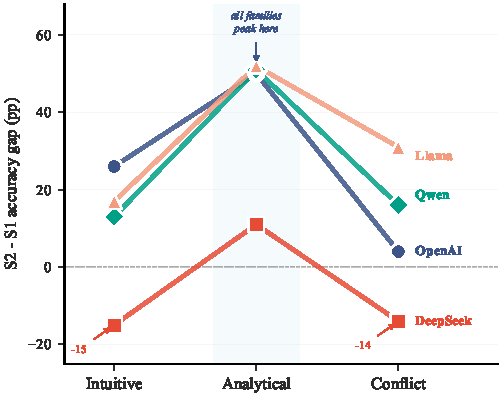
\includegraphics[width=0.82\columnwidth]{figures/fig4_multi_model.pdf}}
\caption{System~2 minus System~1 accuracy gaps across four model families. All families show the predicted pattern: large gaps on analytical tasks (+24 to +53 points), near-zero (raw $-8$ to +10 points) intuitive gaps that turn uniformly positive once the WinoGrande hedging artefact (Section~\ref{sec:factorial-results}) is excluded, and moderate positive gaps on conflict tasks (+6 to +26 points) once option positions are randomised and all 50 novel items are included by stratified sampling.}
\label{fig:multimodel}
\end{figure}

Across all families, the S2--S1 gap was largest on analytical tasks (range:
+24.0 to +53.0 points) and positive for all four families. Intuitive gaps varied across a narrower range ($-8.0$ to +10.0 points) and remained much smaller than the analytical gap for every family. The negative OpenAI intuitive gap ($-8$ points) is, however, an artefact of WinoGrande CoT hedging rather than a genuine CoT-hurts-pattern-matching effect: excluding WinoGrande, every family shows a positive intuitive gap ($+3.7$, $+6.2$, $+16.3$, $+8.8$ for OpenAI, DeepSeek, Qwen, Llama; mean $+8.8$ points). The discussion in Section~\ref{sec:cross-model-robustness} returns to this caveat. On conflict tasks, all four families now show a positive S2--S1 gap (range: +6.0 to +26.0 points). Unlike the raw TruthfulQA-only gaps typically reported in the literature, these numbers reflect a 50/50 stratified sample of classic TruthfulQA items and memorisation-resistant novel items with randomised option positions (see Section~\ref{sec:novel-conflict-results}). This replicates the task-selective pattern documented in the factorial ablation across architectures and training regimes, indicating that the dual-process pattern is consistent across providers and is not an artifact of a single model family.

\subsection{Novel vs.\ Classic Conflict Tasks}
\label{sec:novel-conflict-results}

The conflict category combines TruthfulQA items with 50 novel CRT-style items. To remove two sources of bias identified during analysis, we (i) use \textit{stratified sampling} that forces all 50 novel items into every 200-item conflict sample (filled with 150 random TruthfulQA items), and (ii) randomise MCQ option positions per item with a deterministic per-item seed, so that ``the correct answer is always A'' cannot shortcut evaluation. All eight factorial conditions see the same post-shuffle option layout, making across-condition comparisons valid (Table~\ref{tab:novel-conflict}).

\begin{table}[t]
\caption{Conflict task accuracy (\%) under different comparisons, with option positions randomised and 50 novel + 150 classic items per condition.}
\label{tab:novel-conflict}
\centering
\begin{tabular}{lcccc}
\toprule
Comparison & S1 & S2 & $\Delta$ & $p$ \\
\midrule
C1 vs.\ C8 (canonical) & 58.0 & 73.5 & $+15.5$ & $.001$ \\
C5 vs.\ C8 (same model) & 74.5 & 73.5 & $-1.0$ & $.820$ \\
\bottomrule
\end{tabular}
\end{table}

The canonical C1 vs.\ C8 conflict gap now reaches significance ($+15.5$ points, $t(398) = -3.30$, $p = .001$, $d = 0.330$), driven entirely by model capacity (see Table~\ref{tab:main-effects}: Model effect on conflict $= +15.0$). The same-model C5 vs.\ C8 comparison remains non-significant ($p = .820$), indicating that within GPT-4o, temperature and CoT do not meaningfully change conflict performance. Separating the sample by item source reveals a dramatic training-data contamination signature: on C1, novel-item accuracy (32.0\%, $n = 50$) was less than half the classic TruthfulQA accuracy (66.7\%, $n = 150$); on C8 the gap narrowed but remained substantial (novel 62.0\% vs.\ classic 77.3\%). The larger model generalises more broadly, while the smaller one relies more heavily on surface recall. Disaggregating by novel subcategory (C1 $\to$ C8, $n=10$ items each, paired-bootstrap 95\% CIs): CRT $+30\%$ [$0, +60$], base-rate neglect $+40\%$ [$+10, +70$], conjunction fallacy $+80\%$ [$+50, +100$], biomedical Bayesian reasoning $+10\%$ [$-20, +40$], and other heuristic-and-bias items $-10\%$ [$-30, 0$]. Conjunction-fallacy items show the largest and statistically cleanest S2 $-$ S1 gap; biomedical and mixed-bias items are underpowered at $n=10$ and should be interpreted cautiously.

\subsection{Biomedical Validation on MedQA-USMLE}
\label{sec:medqa}

To substantiate the paper's biomedical framing, we re-ran C1, C5, and C8 on 100 items from the MedQA-USMLE 4-option test set~\cite{Jin2021}. Accuracies: C1 $= 70.0\%$, C5 $= 92.0\%$, C8 $= 88.0\%$; model-capacity effect $+22.0$ ($t(198) = -4.11$, $p < .001$, $d = 0.581$); canonical S2 $-$ S1 gap $+18.0$ ($p = .002$, $d = 0.451$); within-GPT-4o CoT effect $-4.0$ ($p = .348$, n.s.). Same-model TER is negative ($-0.015$ at $1.96\times$ token cost), mirroring the intuitive-task pattern rather than the analytical one: USMLE vignettes behave as \textit{pattern retrieval} for GPT-4o --- scale matters, deliberation does not. Overconfidence on MedQA is far lower than on general benchmarks (C5 gap $= +0.9\%$, C8 $= +2.6\%$, vs.\ $+26.6\%$ and $+15.3\%$ general), consistent with strong medical pre-training. Clinical triage dominated by USMLE-style pattern retrieval is well-served by capable zero-shot; CoT should be reserved for tasks requiring novel inference.

\subsection{Qualitative Comparison with Human Cognition}
\label{sec:human-comparison}

We offer a \textit{qualitative} comparison against published human effects. Human S2--S1 gaps are approximate ranges drawn from cognitive-psychology studies on intuitive pattern tasks ($\sim$$+3\%$), syllogistic and arithmetic reasoning ($\sim$$+25\%$), and CRT / base-rate / framing / conjunction items ($\sim$$+39\%$)~\cite{Frederick2005, Stanovich2000, Pennycook2015}, typically operationalised as time-pressure vs.\ untimed conditions. These are not matched experiments, and we do not claim equivalence of constructs.

Averaged across the four model families, the raw LLM category-level gaps are intuitive $+2.3\%$, analytical $+43.2\%$, and conflict $+15.8\%$; all three share the sign of the corresponding human gap. The raw intuitive magnitude is coincidentally close to the human value ($+2.3\%$ vs.\ $\sim$$+3\%$), but this closeness is misleading because the raw LLM intuitive gap is suppressed by the WinoGrande hedging artefact (Section~\ref{sec:factorial-results}): excluding WinoGrande raises the LLM intuitive gap to $+8.8\%$, about $3\times$ the human value, so in fact LLMs gain \textit{more} from deliberation on pattern-matching tasks than humans do. The analytical and conflict magnitudes also diverge from human, and the rank order differs: humans show their largest gap on conflict tasks, while LLMs show theirs on analytical tasks and only a moderate gap on conflict. One plausible reason for the smaller LLM conflict gap is that LLMs have encountered classic conflict items during pre-training, so an intuitive lure is less likely to dominate their first-pass response, an interpretation supported by the ${\sim}35$-point novel-vs-classic gap observed on C1 (Section~\ref{sec:novel-conflict-results}). A rigorous comparison would require testing humans and LLMs on identical tasks under matched conditions, which we leave to future work.

\subsection{Token Efficiency}
\label{sec:token-efficiency}

Token efficiency analysis reveals task-type-dependent returns on computational investment (Fig.~\ref{fig:cot-interaction}). All TER numbers below are computed on the primary C5 vs.\ C8 contrast (same GPT-4o model; Table~\ref{tab:main-results}), where CoT responses use $2.40\times$ as many tokens as zero-shot responses.

\begin{figure}[t]
\centerline{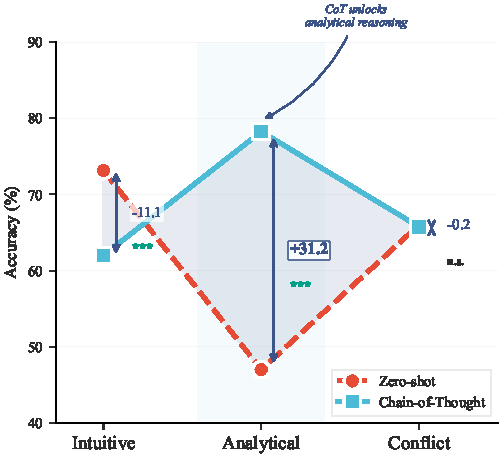
\includegraphics[width=0.82\columnwidth]{figures/fig6_cot_interaction.pdf}}
\caption{Prompt $\times$ Task Category interaction. Mean accuracy under zero-shot vs.\ chain-of-thought, averaged over all model $\times$ temperature cells. CoT produces a large gain on analytical tasks ($+31.2$, $p < .001$); a raw decrement on intuitive tasks ($-11.1$, $p < .001$) roughly half of which is driven by CoT-induced hedging on WinoGrande (Section~\ref{sec:factorial-results}); and no change on conflict tasks ($-0.2$, n.s.).}
\label{fig:cot-interaction}
\end{figure}

On analytical tasks, the Token Efficiency Ratio was
0.118 (percentage points gained per additional token), with a Marginal Accuracy Gain of +26.5\% for an additional ${\sim}225$ tokens. On intuitive tasks, raw TER was slightly negative ($-0.009$), but this number is also contaminated by the WinoGrande CoT hedging artefact (Section~\ref{sec:factorial-results}): recomputing the intuitive C5 vs.\ C8 contrast on the remaining four intuitive benchmarks flips the accuracy delta from $-2.0$ to $+2.3$ points and the TER from $-0.009$ to $+0.011$, so the honest reading is that CoT is roughly TER-neutral on genuine pattern-matching tasks rather than actively harmful. On conflict tasks, TER was also slightly negative ($-0.004$), reflecting a small accuracy \textit{decrement} per additional token in the same-model C5 vs.\ C8 contrast.

System~1-like configurations are equally or slightly more token-efficient on genuine pattern-matching tasks (once WinoGrande hedging is set aside), while System~2-like configurations provide meaningful accuracy gains on analytical tasks that justify the additional token cost.

\subsection{Trial-Level Visualization}

Fig.~\ref{fig:trial-matrix}(a) displays per-source accuracy for all 4{,}800 factorial trials across the eight conditions. The barcode-like pattern reveals the two independent main effects at the individual-trial level. Along the \textit{prompting} axis (comparing C1$\leftrightarrow$C2, C3$\leftrightarrow$C4, C5$\leftrightarrow$C6, C7$\leftrightarrow$C8), the Analytical section (GSM8K, LogiQA) transitions from predominantly red (incorrect) under zero-shot to predominantly green (correct) under CoT, while the Intuitive section shows a reddening that is driven disproportionately by WinoGrande (where CoT-induced hedging collapses accuracy from $\approx 50\%$ to $\approx 2\%$; see Section~\ref{sec:factorial-results}), with much smaller drops on HellaSwag ($-9.8$), PIQA ($-4.4$) and SIQA ($-3.7$) and essentially no change on CommonsenseQA. The Conflict section barely moves along the prompting axis. Along the \textit{model-capacity} axis (comparing the four mini conditions C1--C4 to the four GPT-4o conditions C5--C8), the Conflict section (Novel in particular) shifts from mostly red to substantially greener, visualising the $+15.0$-point Model main effect on conflict documented in Table~\ref{tab:main-effects}. Panel~(b) reports per-source accuracy for each model family's S1 and S2 runs, showing that the analytical ZS$\to$CoT and mini$\to$large transitions described above reproduce in every provider.

\begin{figure*}[t]
\centerline{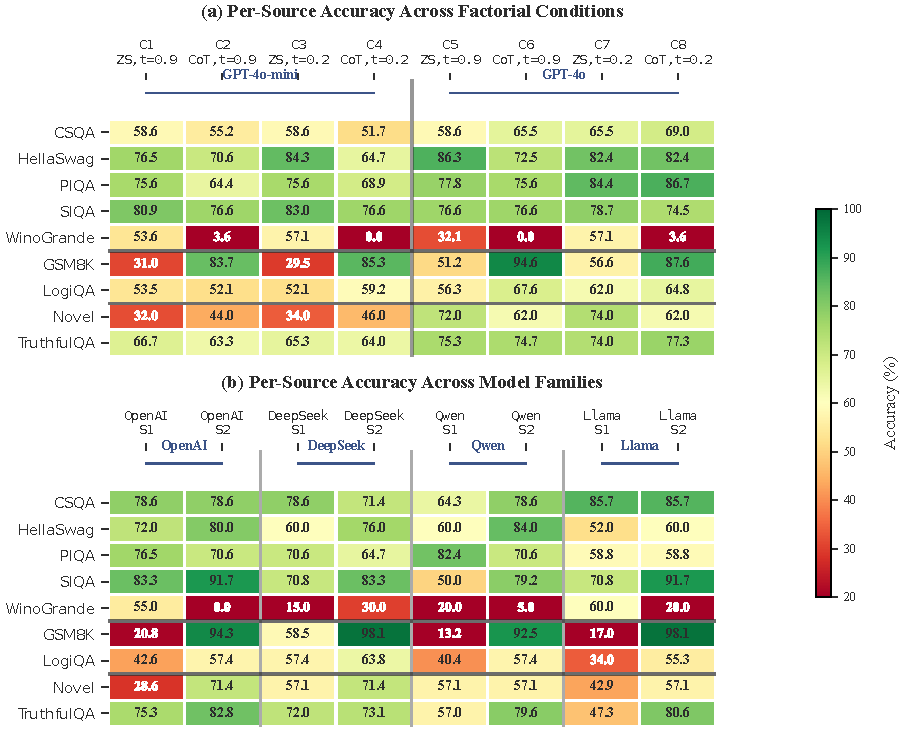
\includegraphics[width=0.75\textwidth]{figures/fig7_trial_matrix.pdf}}
\caption{Per-source accuracy heatmaps (in \%). (a) Factorial ablation: 4{,}800 trials across the 8 conditions C1--C8. CoT dramatically shifts the Analytical section green under CoT conditions; model capacity (mini vs.\ GPT-4o) drives the Conflict section green. (b) Cross-family replication: per-source accuracy for each of the four families' S1 and S2 configurations, showing that the same ZS$\to$CoT and mini$\to$large shifts occur across all four providers.}
\label{fig:trial-matrix}
\end{figure*}


%% ============================================================
\section{Discussion}
\label{sec:discussion}

\subsection{Isolating Dual-Process Factors}

The factorial shows that the System~1/System~2 gap is not simply ``bigger model does better at everything'': model capacity contributes a moderate overall main effect ($\eta^2_p = .012$), prompt a smaller one ($\eta^2_p = .005$), and temperature is null. The Prompt $\times$ Task Category interaction ($\eta^2_p = .036$) is the central finding and survives exclusion of the WinoGrande format artefact (Section~\ref{sec:factorial-results}). We emphasize again that System~1 in humans involves sub-linguistic, pre-attentive processing that has no obvious analogue in autoregressive LLMs; our claim is about behavioral signatures under different configurations, not about underlying mechanisms.

\subsection{Cross-Model Robustness}
\label{sec:cross-model-robustness}

The Prompt $\times$ Task Category pattern documented in the factorial ablation replicates in every one of the four families (Table~\ref{tab:multimodel}): the analytical S2--S1 gap is always large and positive and exceeds the intuitive gap. The $-8$-point intuitive gap for OpenAI and the near-zero gap for Llama warrant caution, however: they are driven by the same WinoGrande hedging effect reported in Section~\ref{sec:factorial-results}. In the multi-family sample (20 WinoGrande items per condition), OpenAI S2 produces 17 hedged ``insufficient context''-style responses on 20 items, and Qwen S2 produces 16 hedged responses; DeepSeek (2) and Llama (2) are much less affected. Excluding WinoGrande, the intuitive S2--S1 gap is positive in \textit{every} family (OpenAI $+3.7$, DeepSeek $+6.2$, Qwen $+16.3$, Llama $+8.8$; mean $+8.8$ vs.\ $+2.3$ with WinoGrande included). The cross-family cross-over that is sometimes invoked as evidence for ``CoT hurts intuitive processing''~\cite{Liu2024} is therefore not robust once the WinoGrande coreference-hedging artefact is controlled for. The remainder of the cross-provider replication (large positive analytical gap, positive conflict gap in every family) is unaffected and is the strongest available evidence that the dual-process patterns are not a GPT-4o-specific artefact.

\subsection{Training Data Contamination}

Under the stratified evaluation, classic TruthfulQA items yield high System~1 (mini) accuracy (66.7\%) despite randomised option positions, well above chance even for the higher-option-count items that dominate TruthfulQA. This suggests substantial training-data memorization. On the 50 novel heuristic-and-bias items that are structurally isomorphic to classic CRT, base-rate, conjunction, Bayesian and related problems but written with novel surface content, System~1 accuracy drops to 32.0\%, a ${\sim}35$-point gap that is difficult to attribute to anything other than recall of classic items from training. The gap narrows sharply for GPT-4o (novel 62.0\% vs.\ classic 77.3\%, a ${\sim}15$-point gap), indicating that the larger model draws more on reasoning and less on recall. These numbers support a concrete recommendation: benchmarks dominated by classic CRT-style items systematically over-estimate LLM resistance to intuitive lures.

\subsection{Implications for Biomedical Decision Support}

These findings provide a principled basis for configuring LLM-based clinical tools:

\textbf{Routine triage and screening.} For pattern-matching tasks (identifying abnormal lab values, flagging critical results, initial symptom screening), System~1-like configurations (smaller models, zero-shot prompting) are adequate and more cost-effective. The factorial analysis shows that, on intuitive tasks, CoT prompting produces no accuracy gain over zero-shot despite a $2.40\times$ token cost: raw deltas are $-11.1$ points averaged over cells and $-2.0$ points for the same-model C5 vs.\ C8 contrast, but these numbers are inflated by CoT-induced hedging on WinoGrande; the underlying effect on the other four intuitive benchmarks is within ${\pm}3$ points of zero. The practical conclusion is unchanged: the extra CoT tokens do not pay for themselves on pattern-matching tasks, and may additionally introduce unsafe hedging when the input is ambiguous.

\textbf{Complex diagnostic reasoning.} For differential diagnosis, interpreting ambiguous presentations, or evaluating rare conditions, System~2-like configurations (larger models, CoT prompting) provide substantial accuracy gains (+31.2\% on analytical tasks) that justify the additional computational cost.

\textbf{Confidence calibration.} Both configurations overestimate their accuracy (overconfidence gap 15.3\% for System~2 vs.\ 26.6\% for System~1). Brier scores and expected calibration error (ECE, 10-bin) confirm the ordering: C1 Brier $= .351$, ECE $= .262$; C5 Brier $= .291$, ECE $= .186$; C8 Brier $= .184$, ECE $= .116$. System~2 is noticeably better calibrated on every metric but not well calibrated in absolute terms; clinical deployment must therefore treat model confidence as a coarse relative signal and pair it with external calibration or abstention~\cite{Saposnik2016}.

\subsection{Limitations}

(i)~We test behavioral signatures under different configurations, not internal cognitive mechanisms. (ii)~Human baselines are drawn from published studies with different populations and paradigms, so the comparison is qualitative rather than matched. (iii)~CoT mechanically produces more tokens, so we cannot fully separate ``more reasoning'' from ``more output''; further, CoT interacts with the WinoGrande coreference format to induce hedged non-answers (accounting for roughly half of the $-11.1$-point raw intuitive decrement, \S\ref{sec:factorial-results}). Model-reported confidences are elicited through prompting rather than internal probabilities. (iv)~The conflict category is $80\%$ multiple-choice ($160/200$); with option positions randomized per item, and the 50 novel items, though structurally isomorphic to classic problems, are surface-related to them. (v)~The intuitive and analytical trials were not re-run under the stratified/option-randomized protocol (these sources are not positional-bias-prone), and the battery does not cover image-based diagnosis or longitudinal patient reasoning.

%% ============================================================
\section{Conclusion}
\label{sec:conclusion}

A $2 \times 2 \times 2$ factorial ablation reveals a strong Prompt $\times$ Task Category interaction: CoT disproportionately benefits analytical tasks ($+31.2$ points) and produces a smaller, format-sensitive decrement on intuitive tasks (raw $-11.1$, of which about half is WinoGrande CoT-induced hedging; ${\sim}-5$ on the other intuitive benchmarks). This directional asymmetry is predicted by dual-process theory but not guaranteed by the design, and it generalises across four LLM families. A 100-item MedQA-USMLE validation shows $+22$ points from model scaling and no CoT benefit within GPT-4o, indicating that USMLE vignettes behave as pattern-retrieval. For biomedical informatics, these findings support configuring LLM-based decision support with efficient System~1-like settings for routine pattern-retrieval and thorough System~2-like settings for complex diagnostic reasoning where accuracy and calibrated confidence both matter.

\paragraph*{Code and data availability}
All task datasets, model prompts, trial-level JSON outputs for the 4{,}800-trial factorial and the multi-model runs, statistical analysis scripts, and figure-generation code will be released at a public GitHub repository upon acceptance. The MedQA-USMLE evaluation uses the publicly available 4-option test split~\cite{Jin2021}.

\bibliographystyle{IEEEtran}
% Tighten inter-item spacing in bibliography (line spacing only; font size unchanged)
\let\oldthebibliography\thebibliography
\renewcommand{\thebibliography}[1]{%
  \oldthebibliography{#1}%
  \setlength{\itemsep}{0pt}%
  \setlength{\parsep}{0pt}}
\bibliography{references}

\end{document}
